\section*{Minimizing the size of the transmitted messages}

To minimize the forwarded data size, first of all we have to get rid of the names of each data. To keep the data readable for the receiver, we can either use a character to separate each segment of data, or we can agree upon a constant size for each segment of data.

The former code encoded each digit of a decimal number as an ASCII character. It means that the number segment only used 10 out of the 256 possible characters. To compress data, we should utilize all the ASCII characters. One way to do it is to make a character store the number as its address in the 8 bit address table. We basically have to convert the numbers to base 256.

We utilized Labview's \todo{maybe we should move it to implementation} built in flatten to string node, which basically converts numeric data to the correspondent string. For example, it convert an 8 bit integer to the correspondent ASCII character. If the sbRIO and the PC uses the same encoding, they can basically send bitcode as if it was string then decode it by doing a simple conversion.
 
\todo{please specify formally the new and old protocol}

For each arm, the sbRIO must send encoder, potmeter and current measurement data from each of the seven motors. Each data is represented as a 32 bit float. This adds up to 48 bytes of data to be sent each cycle. The described method sends 48 byte long strings not including the header. The former method sends 67 characters for formatting and naming purposes and 96 bytes of numeric data, assuming each double number is sent in 8 digits. It adds up to 163 bytes.

By removing the names from the string and compressing a data, the string can become 70 percents shorter, which is a valuable increase in efficiency.

\begin{figure}[H]
\centering
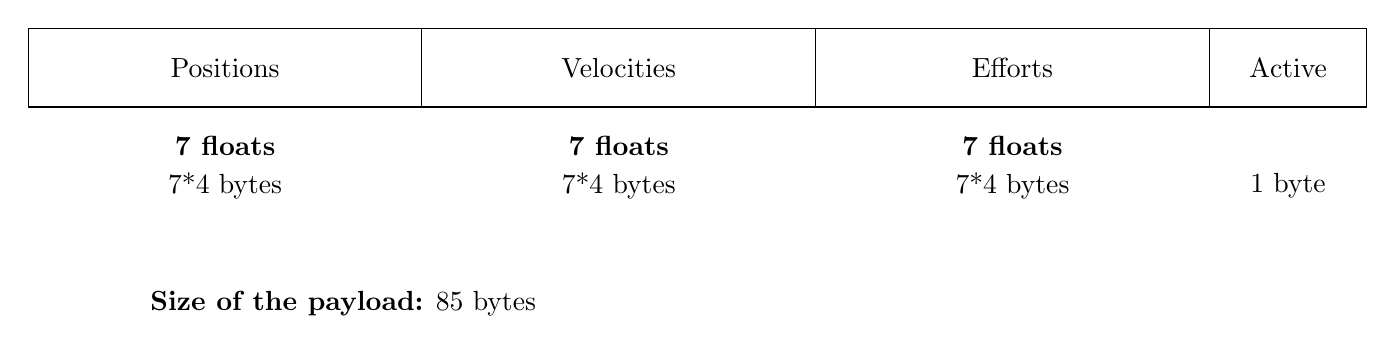
\begin{tikzpicture}

\draw (0,0) rectangle (17,1);
\draw (0,0) rectangle (5,1);
\draw (0,0) rectangle (10,1);
\draw (0,0) rectangle (15,1);

\node at (2.5,0.5) {Positions};
\node at (7.5,0.5) {Velocities};
\node at (12.5,0.5) {Efforts};
\node at (16,0.5) {Active};

\node at (2.5,-0.5) {\textbf{7 floats}};
\node at (7.5,-0.5) {\textbf{7 floats}};
\node at (12.5,-0.5) {\textbf{7 floats}};
%\node at (16,-0.5) {\textbf{n booleans}};

\node at (2.5,-1) {7*4 bytes};
\node at (7.5,-1) {7*4 bytes};
\node at (12.5,-1) {7*4 bytes};
\node at (16,-1) {1 byte};

\node at (4,-2.5) {\textbf{Size of the payload:} 85 bytes}; %I have no idea why i need to put 4 as a coordinate for it to not mess up the rest of the figure
\end{tikzpicture}
\caption{Packet from the sbRIO to ROS for one arm}
\label{received_packet}
\end{figure}

\begin{figure}[H]
\centering
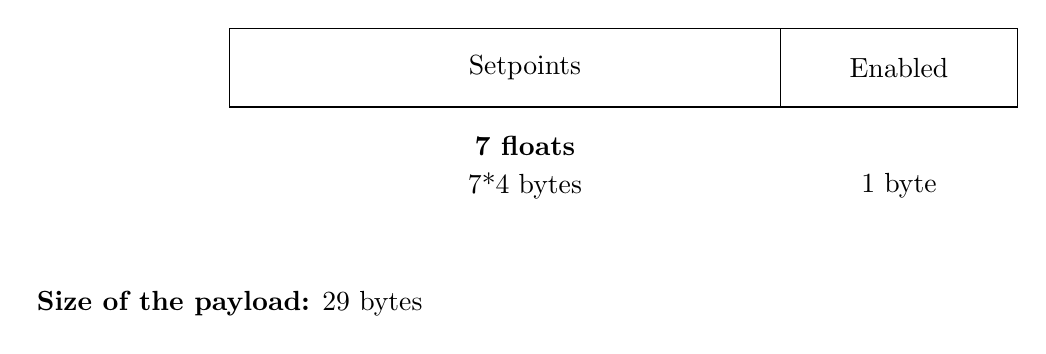
\begin{tikzpicture}

\draw (0,0) rectangle (10,1);
\draw (0,0) rectangle (7,1);

\node at (3.75,0.5) {Setpoints};
\node at (8.5,0.5) {Enabled};

\node at (3.75,-0.5) {\textbf{7 floats}};
%\node at (8.5,-0.5) {\textbf{n booleans}};

\node at (3.75,-1) {7*4 bytes};
\node at (8.5,-1) {1 byte};

\node at (0,-2.5) {\textbf{Size of the payload:} 29 bytes}; 
\end{tikzpicture}
\caption{Packet from ROS to the sbRIO for one arm}
\label{sent_packet}
\end{figure}